\chapter{Partikelfysik} \label{chap:Partikelfysik}

I partikelfysik prøver man at svare på nogle af de mest grundlæggende spørgsmål indenfor naturvidenskaben. Mere præcist kan man sige, at målet med partikelfysik er at svare på de følgende to spørgsmål:
\begin{itemize}
    \item Hvad er universets fundamentale bestanddele, og hvilke egenskaber har disse?
    \item Hvordan velselvirker disse bestanddele med hinanden?
\end{itemize}

Begge disse spørgsmål har fascineret fysikere helt tilbage til de gamle grækere, hvorfor partikelfysikken har en lang og broget historie. Her vil vi dog ikke gå i detalje med den historiske udvikling, da det primære fokus i dette kapitel er at give en introduktion til \emph{Standardmodellen}. 

\section{Standardmodellen}

Standardmodellen er, som navnet antyder, den model fysikkere kloden over betragter, som det bedste bud på hvordan verden fungerer på sit mest grundlæggende plan. For at beskrive, hvordan verdens mindste bestanddele fungerer, skal man kunne beskrive alle typer af vekselvirkninger eller kræfter: elektromagnetisme, den svage kernekraft, den stærke kernekraft og tyngdekraften. I Standardmodellen er elektromagnetisme og de to kernekræfter beskrevet af det, der hedder kvantefeltteori, men det er endnu ikke lykkedes at forene disse tre kræfter med tyngdekraften, som er beskrevet af Einsteins generelle relativitetsteori. Dette tyder på at der må eksistere en mere fuldkommen teori end standardmodellen\footnote{Strengteori og supersymmetri er eksempler på sådanne teorier.}, og selvom der eksisterer mange mulige alternativer, har alle disse store problemer, hvorfor standardmodellen er vores indtil videre bedste bud på en grundlæggende teori for vores univers. 

Standardmodellen beskriver verden som bestående af en række elementarpartikler, der kan kombineres til en hel zoologisk have af partikler, ligesom legoklodser kan kombineres til store og små konstruktioner i alskens farver og former. For at holde styr på medlemmerne af denne zoologiske have opdeles partiklerne i grupper efter deres egenskaber. For at forstå denne opdelingen skal et nyt koncept introduceres.

\textit{Spin} er en fundamental egenskab ved elementarpartikler, der matematisk opfører sig som om, at elementarpartiklerne roterede rundt om sig selv -- ligesom en snurretop. Det er dog kun den matematiske beskrivelse, der er den samme. En rotation kan f.eks. stoppes, hvis man skyder to partikler imod hinanden på den rigtige måde -- det kan spin ikke. Der eksisterer derfor ikke nogen god virklighedsnær analogi for, hvad spin egentligt er, og det betragtes som en elementær egenskab ved en partikel på lige fod med dens elektriske ladning eller dens masse.

I første omgang inddeles partikler i to store grupper, der hedder \emph{bosoner} og \emph{fermioner}\footnote{Opkaldt efter hhv. Satyendra Nath Bose og Enrico Fermi.}. Bosoner defineres som partikler med heltalligt spin, mens fermioner defineres som partikler med halvtalligt spin. Bruger vi notationen $S$ for en given værdi af spin, kan vi altså skrive, at $S_\mathrm{boson} \in \{ 1,2,3,\ldots \}$ og $S_\mathrm{fermion} \in \{ \frac{1}{2},\frac{3}{2},\frac{5}{2},\ldots\}$\footnote{Notationen her betyder, at $S_\mathrm{boson}$ og $S_\mathrm{fermion}$ kan antage alle værdierne i den relevante tuborgklamme: $\{\ldots\}$.}. Den store vigtighed i denne opdeling ligger i selve den matematik, der beskriver, hvordan partiklerne opfører sig. Dette beskrives ikke her, men ikke desto mindre er det vigtigt at kende til. Et resultat af denne matematik er, at fermioner opfylder det, der hedder \emph{Paulis udelukkelsesprincip}, der siger at: "To fermioner ikke kan befinde sig i samme kvantetilstand". Et eksempel på udelukkelsesprincippet er, at elektroner i atomer fordeler sig i forskellige skaller omkring atomkernen og ikke blot samler sig i den skal med mindst energi. Dette ville ellers virke meget naturligt, da fysiske systemer i naturen generelt altid bevæger sig imod den laveste energitilstand. Det er dog ikke tilladt af udelukkelsesprincippet her, idet elektroner har spin $S_\mathrm{elektron} = \frac{1}{2}$, hvorfor de er fermioner.

Da standardmodellen indeholder mange elementarpartikler, er det smart at opskrive et skema, som kan hjælpe med at give et overblik over alle partiklerne. Et sådant skema er vist i figur \ref{fig:standardmodellen}, og det er en rigtig god ide at konsultere dette skema, mens de forskellige partikler i standardmodellen gennemgås nedenfor.
%
\begin{figure}
    \centering
    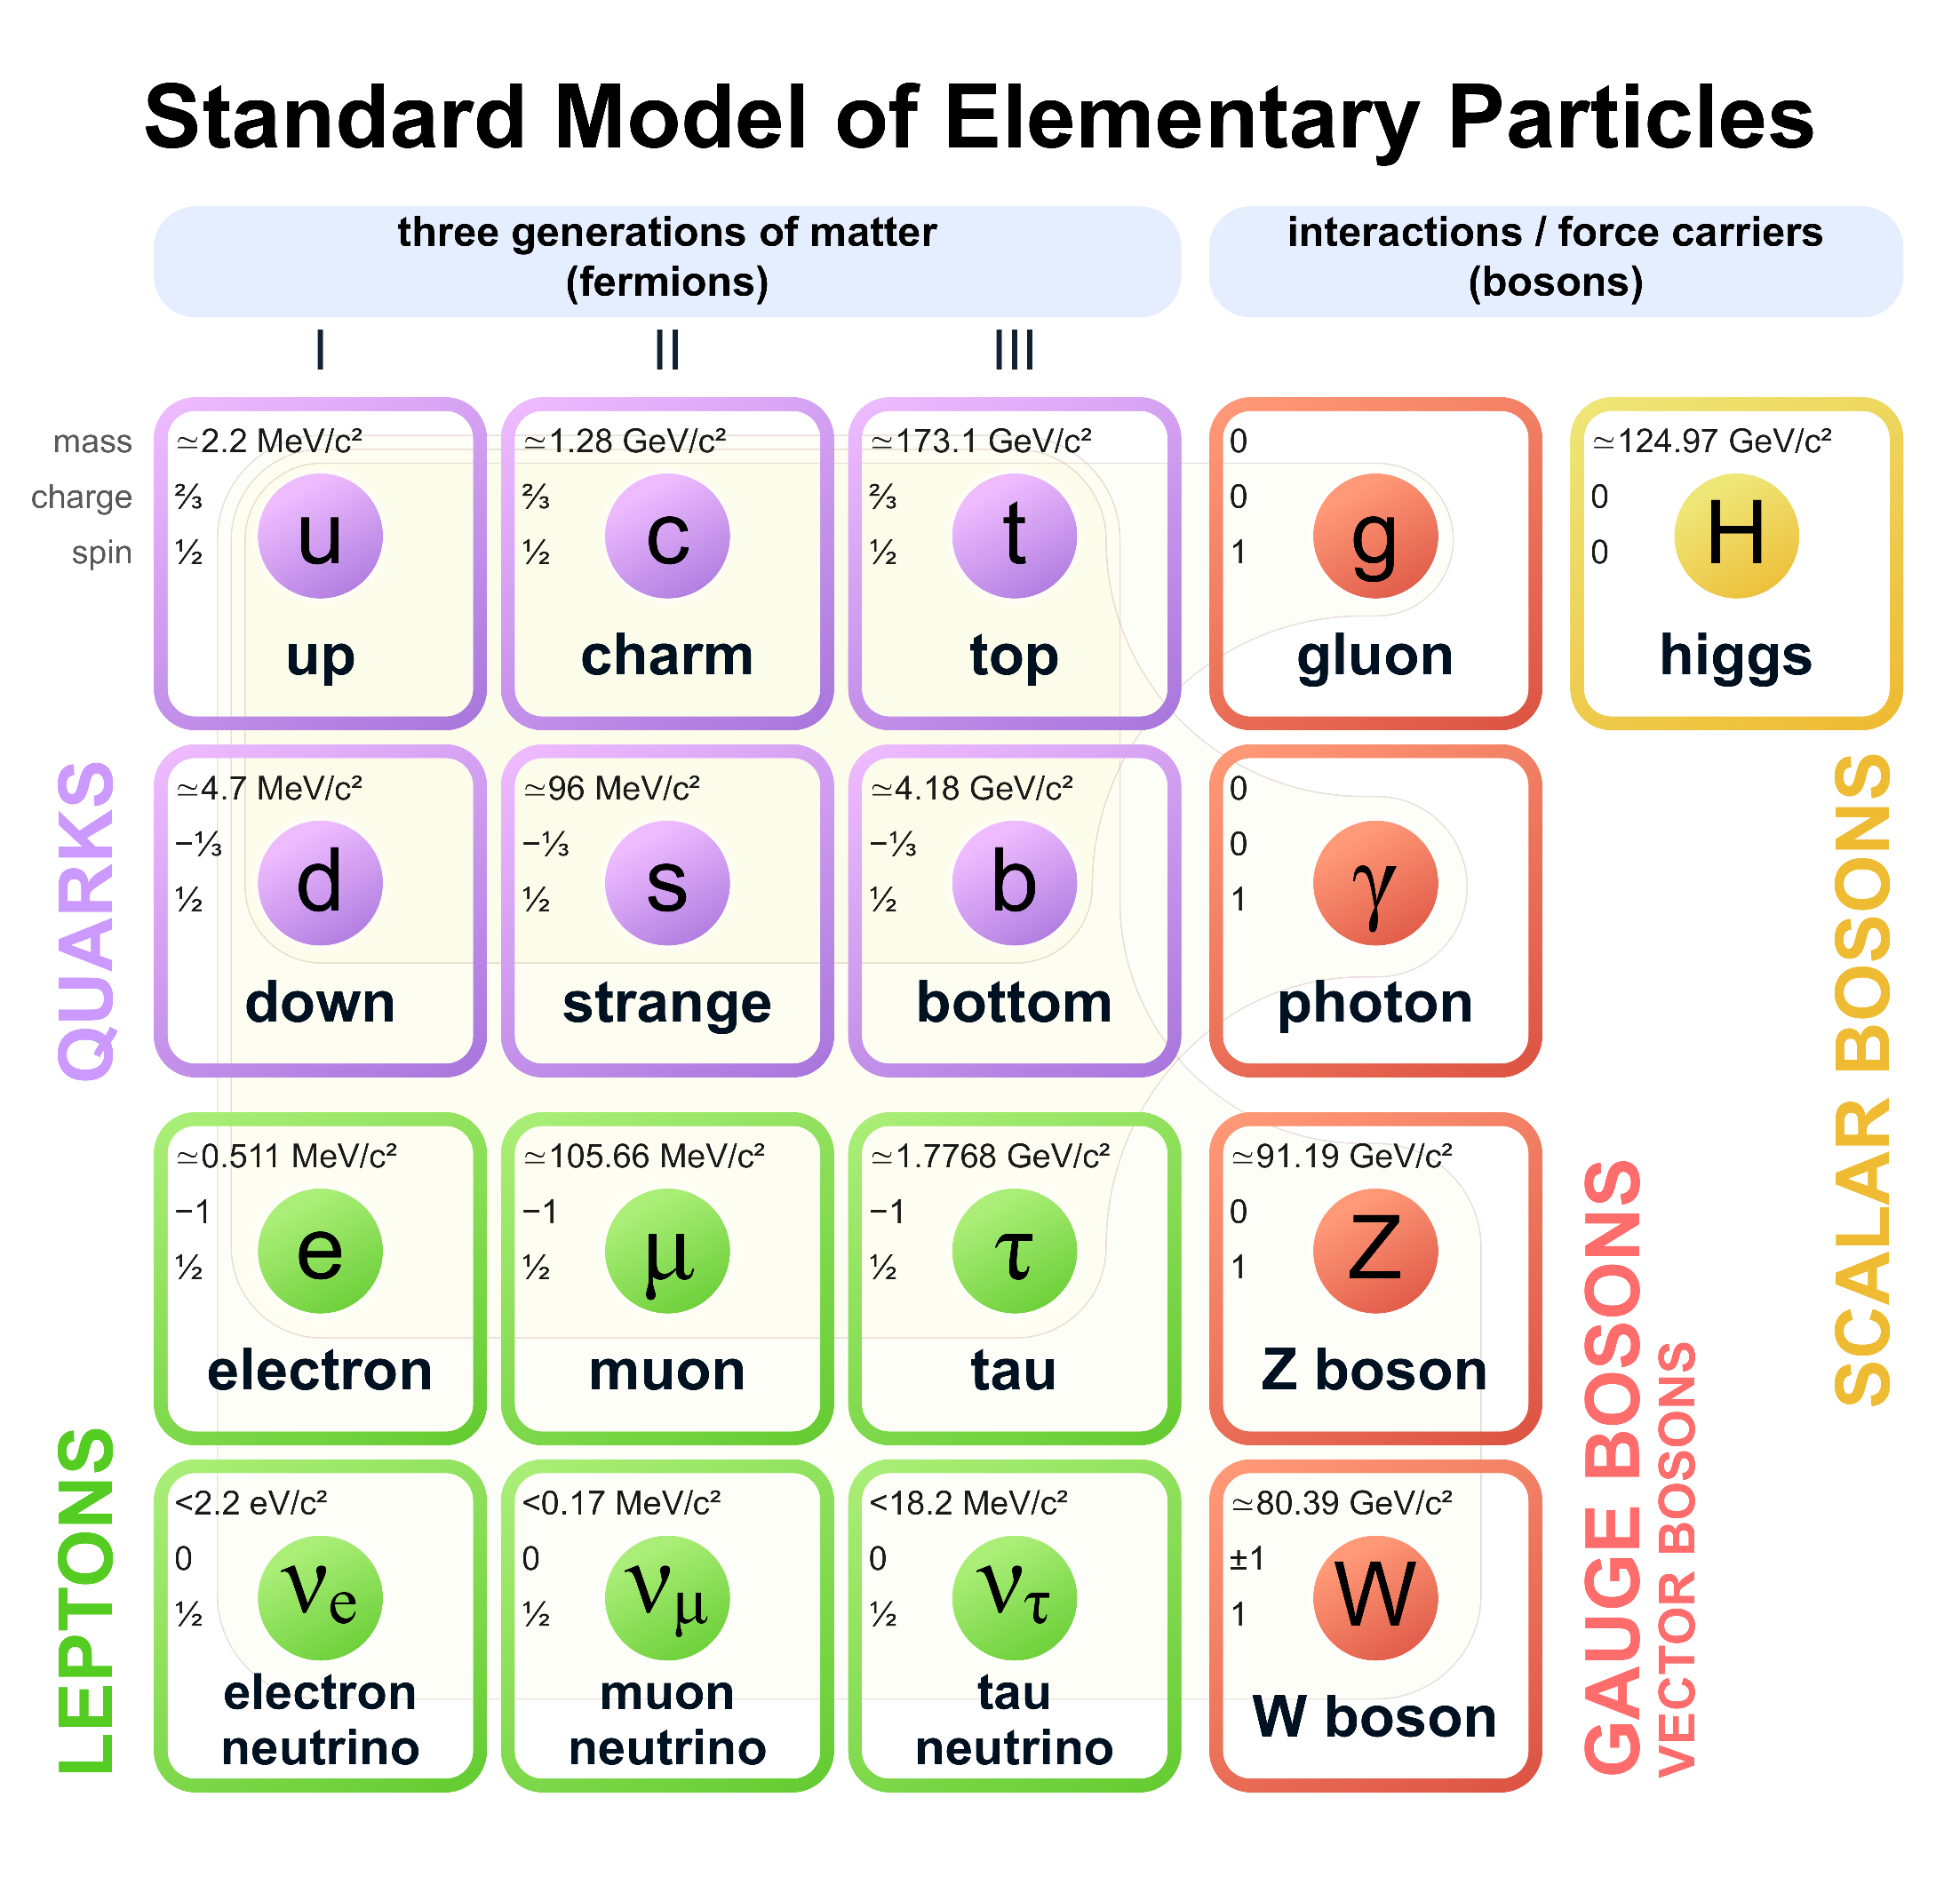
\includegraphics[width=.75\textwidth]{Partikel/figurer/standardmodellen.eps}
    \caption{Skematisk opstilling af elementarpartiklerne hvor deres masse, elektriske ladning og spin fremgår i hver firkants øverste venstre hjørne. Bemærk at enhederne for masse op til et præfiks er \si{\electronvolt\per\clight\squared}, hvilket er den gængse enhed i partikelfysik, da det er smart at kunne relatere massen til energi. Den gruppe hver partikel tilhører er angivet med firkantens farve. Kilde: \cite{StandardModelWikipedia}.}
    \label{fig:standardmodellen}
\end{figure}

\subsection{Fermioner}
Fermioner opdeles i to grupper, \emph{leptoner} og \emph{kvarker}, efter om de har det, man kalder \textit{farveladning}, som afgør om de påvirkes af den stærke kernekraft.

I afsnit \ref{sec:ladning} blev konceptet om elektrisk ladning introduceret, og i resten af kapitel \ref{chap:el} blev ideen om elektriske og magnetiske felter udforsket, samt hvordan ladede partikler vekselvirker med disse. Mere specifikt viser ligningerne \eqref{eq:e-felt_punktpartikel} og \eqref{eq:kraft_fra_e-felt}, at det elektriske felt fra en partikel er proportionalt med partiklens ladning, $\va E \propto q$, og at kraften et elektrisk felt påvirker en partikel med også er proportional med ladningen $\va F \propto q$. Den elektriske ladning kan derfor forstås som et tal, der fortæller hvor meget en partikel vekselvirker med andre partikler igennem den elektromagnetiske kraft. Bemærkelsesværdigt så har elektrisk neutrale partikler den egenskab, at de overhovedet ikke vekselvirker elektromagnetisk -- de danner ikke elektriske eller magnetiske felter, og de er ikke påvirket af sådanne felter fra andre partikler.

Præcis samme ide, som med elektrisk ladning ovenfor, gør sig gældende for farveladning, idet teorien om den stærke kernekraft er konstrueret således, at den minde så meget som muligt om den elektromagnetiske kraft, da netop denne kraft fungerer så godt i kvantefeltteori.

\subsubsection{Leptoner} \label{sec:lepton}
De partikler som ingen farveladning har, kaldes \emph{leptoner}, og den mest kendte lepton er elektronen, $\mathrm{e}^-$. I standardmodellen har alle partikler det, der kaldes en \emph{antipartikel}. I langt de fleste tilfælde er forskellen på en partikel og dens antipartikel, at  fortegnet på deres elektriske ladning er forskellig, mens alt andet (læs "alt andet der er relevant på campen") er ens. Elektronens antipartikel er derfor positivt ladet, og den kaldes en positron, $\mathrm{e}^+$. Udover elektronen eksisterer der også to andre leptoner, som kaldes henholdsvis myonen, $\mu^-$, og tauonen, $\tau^-$, og de har begge hver sin antipartikel, henholdsvis antimyonen, $\mu^+$, og antitauonen, $\tau^+$. Her illustreres et generelt princip i navngivningen af partikler: Med undtagelse af elektronen,  tilføjes anti-- som præfiks til navnet for en partikels antipartikel i stedet for at give den et nyt navn. Forskellen på en elektron, en myon og en tauon er deres masse, $m_\text{e}<m_\mu<m_\tau$ -- resten af deres egenskaber er ens. De har samme spin, elektrisk ladning og farveladning. Denne forskel i masser forklarer, hvorfor atomer i praksis består af elektroner og ikke myoner eller tauoner\footnote{Såkaldte eksotiske atomer, hvor mindst en partikel er erstattet af en anden partikel med samme ladning, eksempelvis en myon i stedet for en elektron, kan dog fremstilles, og er noget der forskes i den dag i dag.}. Kvantefeltteori kombinerer nemlig kvantemekanik med speciel relativitetsteori, hvorfor energi og masse er to sider af samme sag, som det er udtrykt i Einsteins kendte ligning $E = mc^2$. Lidt løst sagt fungerer fysik sådan, at "verden godt kan lide lave energier", og da myoners og tauoners ekstra masse kan omdannes til energi ved at henfalde til elektroner, så er førstnævnte ikke stabile -- lidt ligesom nogle atomkerner henfalder, for på den måde at mindske deres energi. Elektronen, myonen og tauonen, samt deres antipartikler, minder så meget om hinanden, at de i partikelreaktioner opfører sig ens, og derfor kan de betragtes som en mindre undergruppe i den større gruppe af leptoner.\\

Den sidste gruppe af leptoner kaldes \emph{neutrinoer}, der repræsenteres ved symbolet $\nu$\footnote{Her er $\nu$ det græske bogstav ny, og ikke det latinske bogstav $v$.}, og som længe har været meget svære at håndtere i eksperimenter. Det skyldes, at neutrinoer ikke har en elektrisk ladning, og derudover er deres masse \emph{meget} lille. Der findes tre forskellige neutrinoer, der ligesom med $\mathrm{e}^-$, $\mu^-$ og $\tau^-$ kun varierer i forhold til deres masser. Nu kunne man måske tænke, at neutrinoer ikke havde antipartikler, da de ikke har nogen elsktrisk ladning. Neutrinoerne har dog antipartikler, da de har en anden egenskab\footnote{En sådan egenskab er kiralitet, hvilket svarer til håndethed (det fænomen at menneskers højre og venstre hånd ikke er ens men derimod spejlbilleder af hinanden). Kiralitet som fænomen eksisterer også for molekyler, og det er i nogle dele af kemi meget vigtigt. Det er dog ikke vigtigt nok i studiet af partikelreaktioner, til at vi behøver at bekymre os om det på campen.} end elektrisk ladning, som er forskellig mellem partikler og antipartikler. Navngivningen af neutrinoerne følger systemet for de                 tre førnævnte leptoner, hvorfor den letteste neutrino kaldes elektronneutrinoen, $\nu_\mathrm{e}$, den næste kaldes myonneutrinoen, $\nu_\mu$, og den sidst tauneutrinoen, $\nu_\tau$. De elektrisk ladede leptoner er specielle på den måde, at de er de eneste som ikke følger den ellers almindelige konvention om notation for antipartikler, der siger, at en antipartikel skelnes fra dens partikel med en streg. Eksempelvis har antielektronneutrinoen symbolet $\bar{\nu}_\mathrm{e}$.

Neutrinoer er besværlige for eksperimentelfysikere, fordi de hverken har elektrisk ladning eller farveladning, og fordi deres masse, og dermed deres energi, er så lille. Det betyder, at man skal bruge den svage kernekraft for at måle på neutrinoer, men da den er meget svagere end den stærke kernekraft og den elektromagnetiske kraft, er dette yderst vanskeligt. I praksis måler man ofte energien af en neutrino indirekte fra en partikelreaktion. Det gøres ved at måle energien og impulsen på alle de andre reaktionsdeltagere, og så bruge at energi og impuls skal være bevaret for at finde ud af, hvor neutrinoen forsvandt hen, og hvor stor dens energi var. Det at finde neutrinoer svarer derfor lidt til at finde ud af, hvor der har været nåle i en høstak, efter at nålene er blevet fjernet.\\

En sidste gruppering af leptonerne, der er relevant for partikelreaktioner, er opdelingen i leptonfamilier. Lidt løst kan det siges, at alle leptoner hvis navn har noget med elektron at gøre tilhører første familie, dem med myon tilhører anden familie og dem med tauon tilhører den tredje. Elektronens leptonfamilie består altså af elektronen selv, elektronneutrinoen, samt begge partiklers antipartikler. Dette bliver vigtigt i afsnit \ref{sec:partikelreaktioner}.

\subsection{Kvarker}
Opmærksomheden rettes nu mod de fermioner, der har en farveladning forskellig fra 0, også kaldet \emph{kvarker}. Hvor leptonerne var navngivet med græske bogstaver, har kvarkerne af historiske årsager for det meste engelske navne. Kvarkerne kan indeles i to grupper efter deres elektriske ladning. Den første gruppe har elektrisk ladning $q=2e/3$ og består af \emph{opkvarken}\footnote{På engelsk: "upquark".}, u, \emph{charmkvarken}, c, og \emph{topkvarken}, t, mens den anden gruppe har elektrisk ladning $q = -e/3$ og består af \emph{nedkvarken}\footnote{På engelsk: "downquark".}, d, \emph{strangekvarken}, s, og \emph{bottomkvarken}, b. Ligesom leptonerne inddeles i familier, inddeles kvarkerne i generationer efter størrelsesordenen på deres masse. Den første generation er den mest almindelige, og har derfor også danske navne. Den består af opkvarken, u, og nedkvarken, d. Med disse to kvarker kan man danne to partikler, der er bedre kendt end så mange andre -- nemlig protonen og neutronen. Protonen, p, har den elektriske ladning $e$ og består derfor af to opkvarker og en nedkvark, hvilket ofte skrives som, uud. Protonens elektriske ladning er summen af ladningen af kvarkerne den består af, hvorfor
%
\begin{align}
    q_\mathrm{p} = 2q_\mathrm{u} + q_\mathrm{d} = 2\cdot\frac{2}{3}e - \frac{1}{3}e = e.
\end{align}
%
De resterende kvarkgenerationer er den anden generation, som består af c- og s-kvarken, mens den tredje generation består af t- og b-kvarken. Derudover har alle kvarker selvfølgelig også hver deres antipartikel, der noteres og navngives på samme måde som neutrinoerne, hvorfor opkvarkens antipartikel er antiopkvarken og har symbolet $\bar{\mathrm u}$. \\

Nu har vi stiftet bekendtskab med alle de elementarpartikler, som også er fermioner. Der eksisterer mange flere fermioner, men de er kombinationer af de 24, der her er beskrevet, ligesom protoner og neutroner består af op- og nedkvarker. Det er en god ide nu at kigge tilbage på figur \ref{fig:standardmodellen}, og finde de grupperinger der er blevet beskrevet, så man får en god fornemmelse med figuren, og hvordan man kan bruge den til at holde styr på partiklerne.

\section{Bosoner}
For at afslutte beskrivelsen af elementarpartiklerne, mangles nu kun bosonerne, der også kaldes kraftbærere. Dette skyldes, at de så at sige ``bærer informationen`` om de fire fundamentale vekselvirkninger mellem fermionerne. Den mest kendte boson er fotonen, som formidler den elektromagnetiske kraft. Dette gøres ved at en fermion udsender det man kalder en virtuel foton, som absorberes af en anden fermion, hvorved den anden fermion får at vide at den første eksisterer, samt om den helst vil bevæge sig tættere på eller længere væk fra den først fermion -- med andre ord om de to fermioner har samme eller modsat ladning, hvor stor kraften imellem dem er og hvilken retning den peger. At fotonen er virtuel, betyder at den ikke kan observeres eksperimentelt, men at den eksisterer i matematikken, hvor den fortæller de to fermioner om hinandens eksistens. I standardmodellen kan det lidt firkantet siges at bosonerne opgave er at fortæller fermionerne om eksistensen af de andre fermioner og hvordan de skal reagere på eksistensen af disse. Gluonen er kraftbæreren for den stærke vekselvirkling, og i reaktioner opfører den sig ofte ligesom fotonen idet deres egenskaber er meget ens - de er begge spin-1-partikler\footnote{Dette er en gængs måde at sige at en partikel har spin $S=1$, og man siger tilsvarende også at elektroner er spin-1/2-partikler, da de jo har spin $S=1/2$.}, og har ingen masse eller elektrisk ladning -- forskellen i det omfang der er relevant på campen er blot hvilken kraft de formidler. Fotonen og gluonen er elektrisk neutrale og derfor deres egen antipartikel\footnote{De har ikke de andre egenskaber, der skal til for at en antipartikel kan eksistere.}. \\

Udover fotonen og gluonen eksister der tre bosoner, som formidler den svage kernekraft, og de adskiller sig fra de første ved at have masse og to af dem har endda også elektrisk ladning. Der er her tale om den elektrisk neutrale $\mathrm{Z}^0$-boson og de ladede $\mathrm{W}$-bosoner, $\mathrm{W}^+$ og $\mathrm{W}^-$, og disse tre bosoner er meget tunge. Det er faktisk kun topkvarken og Higgsbosonen, som beskrives om lidt, der er tungere, hvilket giver et hint til navnet på den svage kernekraft, som de formidler. Fordi kraftbærerne for den svage kernekraft er så tunge, kræver det store mængder energi at danne disse bosoner, og reaktioner med den svage kernekraft er derfor mindre sandsynlige end reaktioner med den stærke kernekraft eller den elektromagnetiske kraft. \\

Den sidste partikel i standardmodellen er Higgsbosonen, opkaldt efter Peter Higgs, der forudsagde partiklens eksistens tilbage i 60'erne. Higgspartiklens funktion er at give de andre bosoner masse igennem Higgsmekanismen, som ikke uddybes her. Higgsbosonen er meget tung og derfor svær at skabe i et kontrolleret forsøg. Derfor gik der $\sim 50$ år fra dens eksistens blev forudsagt teoretisk til den blev påvist eksperimentelt af fysikere på CERN\footnote{Den partikelaccelerator, man brugte til at finde Higgsbosonen, skyder to stråler af protoner sammen og selve acceleratoren hedder Large Hadron Collider (LHC), fordi den er bygget til at skyde stråler af hadroner mod hinanden og er større end den man havde før.} tilbage i 2013, hvorefter Peter Higgs med flere fik deres Nobelpris.

\section{Hadroner}
Tidligere blev det nævnt at protonen består af to opkvarker og en nedkvark, og protonen er derved et af de mest kendte eksempler på et system sammensat af kvarker, hvilket kaldes \textit{hadroner}. Hadroner opdeles i to grupper; \textit{baryoner}, der består af tre kvarker eller tre antikvarker, og \textit{mesoner}, som består af en kvark og en antikvark. Protonen er derfor en baryon, ligesom dens antipartikel antiprotonen, der består af kvarkerne $\bar{\mathrm u}\bar{\mathrm u}\bar{\mathrm d}$. Man skelner mellem baryoner og mesoner, idet baryoner er fermioner, mens mesoner er bosoner, hvilket er vigtigt for den matematik, der beskriver dem. Årsagerne til dette er komplicerede, men essensen er spin ikke lægges sammen trivielt, da spin er en kvantemekanisk egenskab, som også har en retning\footnote{Det viser sig at sammensætningen af to spin-1/2-partikler give enten en spin-0-partikel eller en spin-1-partikel, men ikke en ny spin-1/2-partikel. Kombinerer man tre spin-1/2-partikler viser det sig at man får enten en ny spin-1/2-partikel eller en spin-3/2-partikel.}. I partikelfysik giver man nye navne til alt hvad man kan slippe afsted med, hvorfor den zoologiske have af partikler er så stor. Det viser sig at op- og nedkvarkerne eksisterer som baryoner på 6 forskellige former, fordi deres spin kan kombineres på forskellige måder, se tabel \ref{tab:baryoner_gen1}. Tabellen illustrerer også at der findes ret så mange hadroner, der alle har mere eller mindre gennemskuelige navne. Heldigvis findes der tabeller over alle kendte mesoner\footnote{\url{https://en.wikipedia.org/wiki/List_of_mesons}} og baryoner\footnote{\url{https://en.wikipedia.org/wiki/List_of_baryons}}, hvor alle relevante egenskaber ved disse partikler også står angivet. Til campens formål er navn, kvarksammensætning, masse og levetid rigeligt, hvor masse og levetid kan bruges til kvalitativt at sige noget om hvor meget energi en partikelreaktion kræver og dermed hvor sandsynlig den er.
%
\def\arraystretch{1.5}
\begin{table}[]
    \centering
    \begin{tabular}{l|ccc}
        Partikelnavn & Partikelsymbol & Kvarksammensætning & Spin \\ \specialrule{.125em}{.1em}{.1em}
        Proton & p & uud & $1/2$ \\ \hline
        Neutron & n & udd & $1/2$ \\ \hline
        Delta(++)baryon & $\Delta^{++}$ & uuu & $3/2$ \\ \hline
        Delta(+)baryon & $\Delta^{+}$ & uud & $3/2$ \\ \hline
        Delta(0)baryon & $\Delta^{0}$ & udd & $3/2$ \\ \hline
        Delta(-)baryon & $\Delta^{-}$ & ddd & $3/2$ \\
    \end{tabular}
    \caption{Baryoner bestående af de tre kvarker fra første generation. Alle seks baryoner har også tilsvarende antipartikler.}
    \label{tab:baryoner_gen1}
\end{table}

\section{Partikelreaktioner} \label{sec:partikelreaktioner}
Ligesom atomer kan reagere med hinanden, hvilket beskrives i kemi, kan partikler også reagere med hinanden. En kemisk reaktion skrives i et reaktionsskema og der gælder visse ting om disse reaktioner -- eksempelvis reagerer hydrogengas med klorgas under dannelse af hydrogenchlorid, der i vandig opløsning kaldes saltsyre,
%
\begin{align}
    \mathrm{H}_2(g) + \mathrm{Cl}_2(g) \longrightarrow 2 \mathrm{HCl}(g).
\end{align}
%
Reaktionspilen udtrykker blandt andet at nogle bestemte størrelser er bevaret under reaktionen, hvilket for en kemisk reaktion er antallet af hvert atom og dermed den samlet masse, energibevarelse, impulsbevarelse og den samlede elektriske ladning\footnote{For kemikere er det irrelevant at der eksisterer andre ladninger end den elektriske (farveladning), hvorfor de med ladningsbevarelse mener bevarelse af elektrisk ladning.}. Lidt det samme gælder for partikelreaktioner, men også en del mere. Da energi og masse er to sider af samme sag, kan masse frit omdannes til energi og omvendt, hvorfor man i fysik her inkluderer masse i energi og regner det som én samlet bevaret størrelse. I kemi bevæger stort set alt sig så langsomt, at den specielle relativitetsteori sjældent er vigtigt, hvorfor kemikerne kan slippe af sted med at lade som om massen er bevaret -- den går dog ikke i partikelreaktioner. Impuls er også bevaret i partikelreakioner, ligesom ladning også er det, dog med den detalje at alle ladninger er bevaret -- både elektrisk ladning og farveladning. Derudover viser det sig at de størrelser, der hedder \textit{baryontal} og \textit{leptontal} er bevaret. Baryontallet, $B$, er antallet af baryoner og leptontallet, $L$, er antallet af leptoner med den detalje at baryoner har baryontal $B=1$ mens antibaryoner har baryontal $B=-1$, mens partikler, der ikke er baryoner har baryontal $B=0$, og ligeledes for leptontallet. Protonen har altså baryontal $B_\mathrm{p} = 1$ mens antiprotonen har baryontal $B_{\bar{\mathrm{p}}} = -1$. Slutteligt er antallet af leptoner fra hver familie i langt de fleste tilfælde bevaret. På campen vil vi kun beskæftige os med reaktioner, der bevarer antallet af medlemmer af hver leptonfamilie. Grunden til at introducere alle disse forskellige grupperinger af elementarpartiklerne er netop at de opfører sig på bestemte måder i partikelreaktioner, hvorfor de gør sådanne reaktioner lettere af overskue, når først man får styr på grupperne. \\

Armeret med bevarelseslovene kan man vurdere om reaktioner kan lade sig gøre eller ej. I praksis vil vi på campen ikke kigge på bevarelse af energi og impuls samt farveladning, da energi- og impulsbevarelse blot sætter krav til hvilket hastigheder, der er mulige, og bevarelse af farveladning er indeholdt i baryontalsbevarelse, som er lettere at arbejde med end farveladningsbevarelse -- med andre ord så er farveladningen bevaret, hvis baryontallet er bevaret. En af de måder atomkerne kan henfalde radioaktivt på, er ved et såkaldt $\beta^-$-helfald, hvor en neutron henfalder til en proton og to leptoner,
%
\begin{align} \label{eq:betaminus}
    \mathrm n \rightarrow \mathrm p + \mathrm{e}^- + \bar{\nu}_\mathrm{e}.
\end{align}
%
Betaminushenfald er observeret eksperimentelt, hvorfor bevarelseslovene er nød til at tillade det, så derfor gennemgås de for at vise at de faktisk er opfyldt.
%
\begin{itemize}
    \item Elektrisk ladningsbevarelse: Neutronen er neutral, hvorfor den samlede ladning af højresiden skal være 0. Protonen har ladning $e$, mens elektronen har ladning $-e$ og neutrinoen er neutral. Da $e-e+0=0$ er ladningen bevaret.
    \item Baryontal: Neutronen er en baryton, hvorfor den har baryontal $B=1$. Ligeledes er protonen en baryon med baryontal $B=1$, mens elektronen og neutrinoen er leptoner med baryontal $B=0$, hvorfor dette er bevaret.
    \item Leptontal: Neutronen og protonen er ikke en leptoner, hvorfor de har leptontal $L=0$. Elektronen er en lepton, hvorfor den har leptontal $L_\text{e} = 1$, mens antielektronneutronien er en antilepton med leptontal $L_{\bar{\nu}_\mathrm{e}} = -1$, hvorfor leptontallet på højre side summer til $L=0$ og dermed er bevaret.
    \item Leptonfamilie: Der dannes en elektron og en antielektronneutrino, som er fra samme leptonfamilie, hvorfor leptontallet for den første familie er bevaret.
\end{itemize}
%
I praksis betyder bevarelsen af leptonfamilierne at når der dannes en elektron, dannes der også en antielektronneutrino og ikke en antimyonneutrino. Det kan dermed også forklares at der dannes en $\bar{\nu}_\mathrm{e}$ og ikke en $\nu_\mathrm{e}$ i $\beta^-$-henfald, da en elektronneutrino ikke bevarer leptontallet. Bemærk at reaktionerne
%
\begin{align}
    n \rightarrow p + \mu^- + \bar{\nu}_\mu, \\
    n \rightarrow p + \tau^- + \bar{\nu}_\tau,
\end{align}
%
også er tilladte. De er dog ikke ligeså sandsynlige som reaktion\eqref{eq:betaminus}, da massen af leptoner fra elektronfamilien er meget mindre end massen af de andre familier. I partikelfysik er det ofte underforstået at enheden for elektriske ladninger er elementarladningen $e$, hvorfor man typisk siger at elektronen har ladning $-1$. Det er lidt noget sjusk, men fysikere er eksperter i at lade så meget som muligt være underforstået, således at man med så få ord som muligt kan kommunikere så meget viden som muligt.

\subsection{Feynmandiagrammer} \label{sec:feynman}
For at overskue partikelreaktioner kan man tegne de såkaldte Feynmandiagrammer, hvilket er en simpel og visuel måde at illustrere reaktioner og overskue om de er tilladte eller ej. Fordi forskellen på bosoner og fermioner er så vigtig, når man regner på partikelfysik, så har de hver deres symbol, og derudover har gluonen sit eget symbol, hvilket er illustreret i figur \ref{fig:Feynmandiagramkomponenter}. Pilene for fermionerne peger til højre, mens pilene på antifermionerne peger til venstre, hvilket også er illustreret i figuren. Akserne for diagrammer er ikke vigtige i den forstand at afstande ikke betyder noget, der er dog en implicit tidsakse, der går fra venstre mod højre. I praksis bruges gluoner oftes til at introducere eksempelvis $\pi^0$-mesoner, der enten har kvarksammensætningen u$\bar{\mathrm u}$ eller d$\bar{\mathrm d}$, for at få reaktioner til at gå op.
%
\begin{figure}
    \centering
    \begin{subfigure}{.2\textwidth}
        \centering
        \begin{tikzpicture}
        \draw[fermion] (0,0) -- (2,0);
        \draw (1,0) node[anchor = north]{fermion};
        \end{tikzpicture}
    \end{subfigure}
    %
    \hspace{5mm}
    %
    \begin{subfigure}{.2\textwidth}
        \centering
        \begin{tikzpicture}
        \draw[fermion] (2,0) -- (0,0);
        \draw (1,0) node[anchor = north]{antifermion};
        \end{tikzpicture}
    \end{subfigure}
    %
    \\
    \vspace{1cm}
    %
    \begin{subfigure}{.2\textwidth}
        \centering
        \begin{tikzpicture}
        \draw[boson] (0,0) -- (2,0);
        \draw (1,0) node[anchor = north]{$\mathrm{W}^\pm$- eller $\mathrm{\mathrm{Z}}^0$-boson};
        \end{tikzpicture}
    \end{subfigure}
    %
    \hspace{5mm}
    %
    \begin{subfigure}{.2\textwidth}
        \centering
        \begin{tikzpicture}
        \draw[photon] (0,0) -- (2,0);
        \draw (1,0) node[anchor = north]{photon};
        \end{tikzpicture}
    \end{subfigure}
    \hspace{5mm}
    %
    \begin{subfigure}{.2\textwidth}
        \centering
        \begin{tikzpicture}
        \draw[gluon] (0,0) -- (2,0);
        \draw (1,0) node[anchor = north]{gluon};
        \end{tikzpicture}
    \end{subfigure}
    \caption{Illustration af de basale symboler i Feynmadiagrammer.}
    \label{fig:Feynmandiagramkomponenter}
\end{figure}
%
I Feynmandiagrammer sker reaktioner i et knudepunkt, der markeres med en prik, og bevarelseslovene gælder for hvert knudepunkt. I disse tegninger bliver bevarelseslovene udtrykt ved at antallet af pile, der peger ind mod et knudepunkt fra venstre, skal pege væk fra samme knudepunkt til højre, den elektriske ladning skal være bevaret i alle knudepunkter, og så skal både baryon- og leptontallet stadig være bevaret. Derved kan et Feynmadiagram for reaktion \eqref{eq:betaminus} tegnes i figur \ref{fig:betaminus}. Læseren opfordres til at tjekke at alle bevarelseslove er opfyldt i begge knudepunkter.
%
\begin{figure}
    \centering
        \begin{tikzpicture}
        \draw[fermion] (-2,0) node[anchor = east]{n} -- (0,0);
        \draw[fermion] (0,0) -- (3,0) node[anchor = west]{p};
        \draw[boson] (0,0) -- (1,1);
        \draw[fermion] (1,1) -- (3,1)node[anchor = west]{$\mathrm{e}^-$};
        \draw[fermion] (3,1.6) node[anchor = west]{$\bar{\nu}_\mathrm{e}$} -- (1,1);
        \draw (0.5,0.5) node[anchor=south east]{$\mathrm{W}^-$};
        \vertex{0,0};
        \vertex{1,1};
        \end{tikzpicture}
    \caption{Feynmandiagram for reaktion \ref{eq:betaminus}.}
    \label{fig:betaminus}
\end{figure}
%
% \section{Regler for Feynman-diagrammer}
% \noindent \emph{Supplement til PN kapitel 4.4}
%
Feynmandiagrammerne er symbolske repræsentationer af processer (henfald eller reaktioner) -- de eneste vigtige aspekter er
\begin{itemize}
    \item Hvordan diagrammet er forbundet. \\
    \item At linjerne deles op i partikler, der går ind i processen, partikler, som kommer ud fra processen, og virtuelle partikler.  Dog skal man klart kunne se om fermionlinjer går til højre eller
venstre, med en klart markeret pil på dem.
\end{itemize}
%
Linjer, som derved går fra et knudepunkt til et andet, repræsenterer virtuelle partikler. Partikler, der ikke deltager i processen, optræder blot som gennemgående linjer. De basale former for knudepunkterne er givet i figur \ref{fig:vertex}. Symbolerne $\ell$, $\nu_{\ell}$ og $q$ står for henholdsvis en ladet lepton (e, $\mu$ eller $\tau$), en neutrino ($\nu_\mathrm{e}$, $\nu_{\mu}$ og $\nu_{\tau}$) og en quark (d, u, s, c, b eller t). Bemærk at W-koblingerne til kvarker involverer d' i stedet for d osv., som betyder at koblingen sker fortrinsvist til, i dette tilfælde, nedkvarken, men at der også kobles til andre kvarker med samme ladning. Koblinger af kvarker fra forskellige generationer er tilladte, men de er undertrykte -- det vil sige at sandsynligheden for at reaktionen, i det knudepunkt, sker er lille.  Kun i knudepunkter hvor W$^-$ eller W$^+$ indgår, kan der ``laves om på'' partikeltypen. Bemærk specielt at da u- og d-kvarker har lille masse vil u$\bar{\mathrm{u}}$- og d$\bar{\mathrm d}$-par kunne dannes af lavenergi gluoner; det er
derfor ``gratis'' at introducere sådanne par i et diagram.  For de andre vekselvirkninger gælder at jo færre knudepunkter, og dermed virtuelle partikler, desto mere sandsynlig er processen. \\

\begin{figure}
    \centering
    \begin{subfigure}{\textwidth}
        \centering
		\begin{tikzpicture}
		    \draw[fermion] (180:1) node[anchor = east]{$l$} -- (0,0);
		    \draw[fermion] (0,0) -- (60:1)node[anchor = south west]{$l$};
		    \draw[photon] (0,0) -- (-60:1)node[anchor = north west]{$\gamma$};
		    \vertex{0,0};
		\end{tikzpicture}
		%
        \hspace{2cm}
        %
		\begin{tikzpicture}
		    \draw[fermion] (180:1) node[anchor = east]{$q$} -- (0,0);
		    \draw[fermion] (0,0) -- (60:1)node[anchor = south west]{$q$};
		    \draw[photon] (0,0) -- (-60:1)node[anchor = north west]{$\gamma$};
		    \vertex{0,0};
		\end{tikzpicture}
        \caption{Elektromagnetiske vekselvirkninger.}
        \label{fig:Feynman_el}
    \end{subfigure}
    %
    \begin{subfigure}{\textwidth}
        \centering
        %
        \begin{tikzpicture}
	    	\draw[fermion] (180:1) node[anchor = east]{$q$} -- (0,0);
		    \draw[fermion] (0,0) -- (60:1)node[anchor = south west]{$q$};
		    \draw[gluon] (0,0) -- (-60:1)node[anchor = north west]{$g$};
		    \vertex{0,0};
		\end{tikzpicture}
        %
        \hspace{3cm}
        %
        \begin{tikzpicture}
		    \draw[gluon] (180:1) node[anchor = east]{$g$} -- (0,0);
		    \draw[gluon] (0,0) -- (60:1)node[anchor = south west]{g};
		    \draw[gluon] (0,0) -- (-60:1)node[anchor = north west]{g};
		    \vertex{0,0};
		\end{tikzpicture}
        %
        \hspace{3cm}
        %
        \begin{tikzpicture}
            \draw[gluon] (0,0) -- (45:1)node[anchor = south west]{g};
            \draw[gluon] (0,0) -- (-45:1)node[anchor = north west]{g};
            \draw[gluon] (0,0) -- (135:1)node[anchor = south east]{g};
            \draw[gluon] (0,0) -- (-135:1)node[anchor = north east]{g};
            \vertex{0,0};
        \end{tikzpicture}
        
        \caption{Stærke vekselvirkninger.}
        \label{fig:Feynman_strong}
    \end{subfigure}
    %
    \begin{subfigure}{\textwidth}
        \centering
        \begin{tikzpicture}
		    \draw[fermion] (0,0) -- (60:1) node[anchor = south west]{$\nu_\mathrm{e}$};
		    \draw[fermion] (180:1)node[anchor = east]{e$^-$} -- (0,0);
		    \draw[boson] (0,0) -- (-60:1)node[anchor = north west]{W$^-$};
		    \vertex{0,0};
		\end{tikzpicture}
		%
        \hspace{3cm}
        %
        \begin{tikzpicture}
		    \draw[fermion] (0,0) -- (60:1) node[anchor = south west]{$\nu_\mu$};
		    \draw[fermion] (180:1)node[anchor = east]{$\mu^-$} -- (0,0);
		    \draw[boson] (0,0) -- (-60:1)node[anchor = north west]{W$^-$};
		    \vertex{0,0};
		\end{tikzpicture}
        %
        \hspace{3cm}
        %
        \begin{tikzpicture}
		    \draw[fermion] (0,0) -- (60:1) node[anchor = south west]{$\nu_\tau$};
		    \draw[fermion] (180:1)node[anchor = east]{$\tau^-$} -- (0,0);
		    \draw[boson] (0,0) -- (-60:1)node[anchor = north west]{W$^-$};
		    \vertex{0,0};
		\end{tikzpicture}
        \caption{Svage vekselvirkninger med leptoner.}
        \label{fig:Feynman_svag_lepton}
    \end{subfigure}
    %
    \begin{subfigure}{\textwidth}
        \centering
        \begin{tikzpicture}
		    \draw[fermion] (180:1) node[anchor = east]{d$'$} -- (0,0);
		    \draw[fermion] (0,0) -- (60:1)node[anchor = south west]{u};
		    \draw[boson] (0,0) -- (-60:1)node[anchor = north west]{W$^-$};
		    \vertex{0,0};
		\end{tikzpicture}
		%
		\hspace{3cm}
		%
		\begin{tikzpicture}
		    \draw[fermion] (180:1) node[anchor = east]{s'} -- (0,0);
		    \draw[fermion] (0,0) -- (60:1)node[anchor = south west]{c};
		    \draw[boson] (0,0) -- (-60:1)node[anchor = north west]{W$^-$};
		    \vertex{0,0};
		\end{tikzpicture}
		%
		\hspace{3cm}
		%
		\begin{tikzpicture}
		    \draw[fermion] (180:1) node[anchor = east]{b'} -- (0,0);
		    \draw[fermion] (0,0) -- (60:1)node[anchor = south west]{t};
		    \draw[boson] (0,0) -- (-60:1)node[anchor = north west]{W$^-$};
		    \vertex{0,0};
		\end{tikzpicture}
        \caption{Svage vekselvirkninger med kvarker.}
        \label{fig:Feynman_svag_kvark}
    \end{subfigure}
    %
    \begin{subfigure}{\textwidth}
        \centering
        \begin{tikzpicture}
		    \draw[fermion] (180:1) node[anchor = east]{$l$} -- (0,0);
		    \draw[fermion] (0,0) -- (60:1)node[anchor = south west]{$l$};
		    \draw[boson] (0,0) -- (-60:1)node[anchor = north west]{Z$^0$};
		    \vertex{0,0};
		\end{tikzpicture}
		%
		\hspace{3cm}
		%
		\begin{tikzpicture}
		    \draw[fermion] (180:1) node[anchor = east]{$q$} -- (0,0);
		    \draw[fermion] (0,0) -- (60:1)node[anchor = south west]{$q$};
		    \draw[boson] (0,0) -- (-60:1)node[anchor = north west]{Z$^0$};
		    \vertex{0,0};
		\end{tikzpicture}
		%
		\hspace{3cm}
		%
		\begin{tikzpicture}
		    \draw[fermion] (180:1) node[anchor = east]{$\nu_l$} -- (0,0);
		    \draw[fermion] (0,0) -- (60:1)node[anchor = south west]{$\nu_l$};
		    \draw[boson] (0,0) -- (-60:1)node[anchor = north west]{Z$^0$};
		    \vertex{0,0};
		\end{tikzpicture}
        \caption{Elektrisk neutrale svage vekselvirkninger.}
        \label{fig:Feynman_svag_neutral}
    \end{subfigure}
    \caption{De basale knudepunkter for (a) den elektromagnetiske vekselvirkning, (b) den stærke vekselvirkning, (c-e) den svage vekselvirkning. Symbolerne $\ell$, $\nu_{\ell}$ og $q$ står for henholdsvis en ladet lepton (e, $\mu$ eller $\tau$), en neutrino ($\nu_\mathrm{e}$, $\nu_{\mu}$ og $\nu_{\tau}$) og en quark (d, u, s, c, b eller t).}
    \label{fig:vertex}
\end{figure}

Der er en frihed i alle knudepunkter i og med at de frit kan roteres, så længe en partikel ombyttes med dens antipartikel, hvis den krydser den imaginære lodrette linje gennem knudepunktet. Figurene \ref{fig:vertex_rot_el} og \ref{fig:vertex_rot_svag} giver nogle eksempler på hvordan man, ud fra de basale knudepunkter, kan finde andre tilladte former for knudepunkter. Yderligere er det også tilladt at skifte fortegn på samtlige partiklers ladning, både elektrisk og farve, i samme Feynmandiagram. % Der er to regler for omformning af et knudepunkt til et andet tilladt knudepunkt: for det f{\o}rste kan man skifte \emph{alle} partikler til antipartikler (og omvendt) i et knudepunkt.  For det andet kan \emph{en} indg{\aa}ende partikel erstattes med en udg{\aa}ende antipartikel (eller de naturlige variationer heraf: en indg{\aa}ende antipartikel erstattes med en udg{\aa}ende partikel, en udg{\aa}ende partikel erstattes med en indg{\aa}ende antipartikel, eller en udg{\aa}ende antipartikel erstattes med en indg{\aa}ende partikel --- en ind/udg{\aa}ende W$^-$ erstattes af en ud/indg{\aa}ende W$^+$, mens fotonen, gluoner og Z$^0$ alle er deres egen antipartikel).
%
\begin{figure}
    \centering
    \begin{tikzpicture}
        \draw[fermion] (180:1) node[anchor = east]{e$^-$} -- (0,0);
		\draw[fermion] (0,0) -- (60:1)node[anchor = south west]{e$^-$};
		\draw[photon] (0,0) -- (-60:1)node[anchor = north west]{$\gamma$};
		\vertex{0,0};
    \end{tikzpicture}
	%
	\hspace{1cm}
	%
	\begin{tikzpicture}
		\draw[fermion] (120:1) node[anchor = south east]{e$^-$} -- (0,0);
		\draw[fermion] (0,0) -- (0:1)node[anchor = west]{e$^-$};
		\draw[photon] (0,0) -- (-120:1)node[anchor = north east]{$\gamma$};
		\vertex{0,0};
	\end{tikzpicture}
	%
	\hspace{1cm}
	%
	\begin{tikzpicture}
	    \draw[photon] (180:1) node[anchor = east]{$\gamma$} -- (0,0);
	    \draw[fermion] (0,0) -- (60:1)node[anchor = south west]{e$^-$};
	    \draw[fermion] (-60:1) node[anchor = north west]{e$^+$} -- (0,0);
	    \vertex{0,0};
	\end{tikzpicture}
	%
	\hspace{1cm}
	%
	\begin{tikzpicture}
		\draw[fermion] (180:1) node[anchor = east]{e$^+$} -- (0,0);
		\draw[photon] (0,0) -- (60:1)node[anchor = south west]{$\gamma$};
		\draw[fermion] (-60:1) node[anchor = north west]{e$^+$} -- (0,0);
		\vertex{0,0};
	\end{tikzpicture}
    \caption{Eksempel på hvordan det samme basale (elektromagnetiske) knudepunkt kan omformes udfra de to regler nævnt i teksten.}
    \label{fig:vertex_rot_el}
\end{figure}

\begin{figure}[ht]
    \centering
    \begin{tikzpicture}
		\draw[fermion] (180:1) node[anchor = east]{e$^-$} -- (0,0);
		\draw[fermion] (0,0) -- (60:1)node[anchor = south west]{$\nu_\mathrm{e}$};
		\draw[boson] (0,0) -- (-60:1)node[anchor = north west]{W$^-$};
		\vertex{0,0};
	\end{tikzpicture}
	%
	\hspace{1cm}
	%
	\begin{tikzpicture}
		\draw[fermion] (120:1) node[anchor = south east]{e$^-$} -- (0,0);
		\draw[fermion] (0,0) -- (0:1)node[anchor = west]{$\nu_\mathrm{e}$};
		\draw[boson] (0,0) -- (-120:1)node[anchor = north east]{W$^+$};
		\vertex{0,0};
	\end{tikzpicture}
	%
	\hspace{1cm}
	%
	\begin{tikzpicture}
		\draw[boson] (180:1) node[anchor = east]{W$^-$} -- (0,0);
		\draw[fermion] (0,0) -- (60:1)node[anchor = south west]{e$^-$};
		\draw[fermion] (-60:1) node[anchor = north west]{$\bar{\nu}_e$} -- (0,0);
		\vertex{0,0};
	\end{tikzpicture}
	%
	\hspace{1cm}
	%
	\begin{tikzpicture}
		\draw[fermion] (180:1) node[anchor = east]{e$^+$} -- (0,0);
		\draw[boson] (0,0) -- (60:1)node[anchor = south west]{W$^+$};
		\draw[fermion] (-60:1) node[anchor = north west]{$\bar{\nu}_e$} -- (0,0);
		\vertex{0,0};
	\end{tikzpicture}
    \caption{Eksempel på hvordan det samme basale (svage) knudepunkt kan omformes udfra de to regler nævnt i teksten.}
    \label{fig:vertex_rot_svag}
\end{figure}\\

Et af knudepunkterne i figur \ref{fig:vertex_rot_el} er så speciel at den, og dens modsatte proces, har fået særlige navne. En særlig egenskab ved partikel-antipartikelpar er at de vekselvirker elektromagnetisk med hinanden således at de så at sige ``går ud med hinanden'' og bliver til en foton, hvis de støder sammen. Denne proces kaldes annihilation og er illustreret for et elektron-positronpar i figur \ref{fig:annihilation}. Da knudepunkter i Feynmandiagrammer kan roteres, hvor der tages hensyn til korrekt ændring af ladninger, kan den modsatte proces også kan forekomme. Den kaldes pardannelse og er for elektron-positronparret illustreret i figur \ref{fig:pardannelse}.
%
\begin{figure}
    \centering
    \begin{subfigure}{.47\textwidth}
        \centering
        \begin{tikzpicture}
        \draw[fermion] (-120:1) node[anchor = north east]{$\mathrm{e}^-$} -- (0,0);
        \draw[fermion] (0,0) -- (120:1) node [anchor = south east]{$\mathrm{e}^+$};
        \draw[photon] (0,0) -- (1,0)node [anchor = west]{$\gamma$};
        \vertex{0,0};
        \end{tikzpicture}
        \caption{Annihilation af en elektron og en positron.}
        \label{fig:annihilation}
    \end{subfigure}
    %
    \hspace{5mm}
    %
    \begin{subfigure}{.47\textwidth}
        \centering
        \begin{tikzpicture}
        \draw[fermion] (-60:1) node[anchor = north west]{$\mathrm{e}^+$} -- (0,0);
        \draw[fermion] (0,0) -- (60:1) node [anchor = south west]{$\mathrm{e}^-$};
        \draw[photon] (0,0) -- (-1,0)node[anchor = east]{$\gamma$};
        \vertex{0,0};
        \end{tikzpicture}
        \caption{Pardannelse af en elektron og en positron.}
        \label{fig:pardannelse}
    \end{subfigure}
    \caption{Feynmadiagrammer for annihilation og pardannelse af et elektron-positronpar.}
    \label{fig:annihilation_pardannelse}
\end{figure}

\subsection{Reaktionssandsynlighed} \label{sec:reaktionssandsynlighed}
I partikelfysik kan alle reaktioner, som man kan tegne et Feynmandiagram for, ske i virkeligheden, men der er dog forskel på, hvor sandsynlige de er. Hvis man vil regne sandsynligheden for at en reaktion forekommer, så skal man tage højde for alle mulige måder hvorpå reaktionen kan forekomme. Teknisk set er der uendelig mange måder, hvorpå en reaktion kan forekomme, idet kvarker mere eller mindre frit kan udsende og optage virtuelle gluoner. Da gluonerne er virtuelle partikler, er der tale om flere måder at opnå samme reaktion og man skal derfor i princippet regne alle mulighederne med. Der eksisterer dog nogle gode tommelfingerregler for, hvad der gør reaktioner mere eller mindre sandsynlige. I punktform er disse retningslinjer:
%
\begin{itemize}
    \item Jo flere knudepunkter en reaktion indeholder, desto mindre sandsynlig er reaktionen.
    \item Stærke vekselvirkninger er mere sandsynlige end elektromagnetiske.
    \item Elektromagnetiske vekselvirkninger er mere sandsynlige end svage vekselvirkninger.
    \item Svage vekselvirkninger, der kobler kvarker af samme generation, er mere sandsynlige end svage vekselvirkninger, der kobler kvarker af forskellige generationer.
    \item Jo tungere partikler, der indgår i reaktionen, desto mindre sandsynligt er reaktionen.
    \item Den svage vekselvirkninger er så usandsynlig at to eller flere svage vekselvirkninger  meget sjældent sker.
\end{itemize}
%
At nogle vekselvirkninger er mere sandsynlige end andre, er svært at forklare, da det langt hen ad vejen er bestemt ved eksperimenter. Et argument for at svage vekselvirkninger er mindre sandsynlige end de to andre er at de bosoner, der formidler den svage vekselvirkning, $\mathrm{Z}^0$ og $\mathrm{W}^\pm$, er meget tunge, mens gluonen og fotonen er masseløse. Det forklarer ikke hvorfor den stærke vekselvirkning er mere sandsynlig end den elektromagnetiske, men dog hvorfor den svage er speciel. Det er dog relativt simpelt at forklare at det er mere sandsynligt at reaktioner foregår med lette partikler end tunge, idet energi og masse er to sider af samme sag, så jo tungere en partikel man bruger i sit Feynmandiagram, desto mere energi skal der være tilstede, for at denne partikel dannes -- også selvom den blot er virtuel. Når man tæller antallet af vekselvirkninger, så tæller man antallet af bosoner og ikke antallet af knudepunkter. Der er derfor $1$ svag vekselvirkning i figur \ref{fig:betaminus}, da der er $1$ $\mathrm{W}^-$ boson mellem to knudepunkter. Hvert knudepunkt har en sandsynlighed for at forekomme, og sandsynligheder er beskrevet ved tal mellem $0$ og $1$. Har man flere knudepunkter, så er sandsynligheden for at reaktionen forekommer, produktet af de individuelle sandsynligheder. Ganger man to tal sammen, der begge er mindre end $1$, får man et tal, som er mindre end begge de to tal, ergo mindskes sandsynligheden for at en reaktion forkommer, når antallet af knudepunkter øges. Dette er det samme som sandsynligheden for at få et bestemt udfald ved et spil plat og krone. Slår man $2$ gange, er sandsynligheden for at alle mønterne giver krone, større end hvis man slår $3$ gange. Partikelreaktioner fungerer på samme måde, hvor det er mere sandsynligt at $2$ vekselvirkninger sker, end at $3$ vekselvirkninger sker.

\nocite{cramerandersenUniversetsByggestenModerne2013}